% Plantilla de presentación UC3M / Instituto de Salud Carlos III.
% Demo de los tres tipos de diapositiva (normal, dos columnas, dos filas),
% del modo matemático, de las subsecciones y de los enlaces.
%
% El contenido es un ejemplo inventado (detección de anomalías en series de
% sensores); las cifras no proceden de ningún experimento real.
%
% Compilar:  make      (latexmk -lualatex, dos pasadas por el índice)
\documentclass[aspectratio=169,9pt]{beamer}
\usetheme{uc3m}

\usepackage[spanish,es-noquoting]{babel}
\usepackage{booktabs}

\title{Detección de anomalías en series temporales de sensores}
\date{Septiembre 2026}
\author{Raúl Aguilar Arroyo\\Nombre Apellido\\Nombre Apellido}

\begin{document}

\begin{frame}[plain,noframenumbering]
  \titlepage
\end{frame}

\section{Dos columnas}

% ------------------------------------------------ 1. un párrafo por columna --
\subsection{Texto}

\begin{frame}{Un párrafo por columna}
\begin{twocols}
  El detector por ventana deslizante compara cada lectura con las de su
  entorno inmediato: la referencia se calcula sobre la propia serie, de modo
  que todo lo que varía lentamente queda absorbido por la media móvil.
\nextcol
  Esto elimina la necesidad de un modelo explícito de la señal y neutraliza
  las derivas lentas del sensor, a costa de perder las anomalías que se
  extienden más allá del tamaño de la ventana.
\end{twocols}
\end{frame}

% ------------------------------------------- 2. con cabecera y varios párrafos --
\begin{frame}{Con cabecera y varios párrafos}
\begin{twocols}
  \panelheading{Contexto}

  Los métodos clásicos de detección de anomalías en series temporales
  ajustan un modelo de la señal y señalan como anómalas las lecturas que se
  alejan de la predicción.

  Su coste principal es el ajuste del modelo, que hay que repetir para cada
  sensor y revisar cuando cambian las condiciones de operación, con una
  ventana de calibración típica de \textbf{[t-30, t-1]}.

  Concluyen que la mayor parte de las anomalías reales son puntuales y de
  corta duración.
\nextcol
  \panelheading{Este trabajo}

  Aquí se comprueba si empleando \textbf{únicamente} una media móvil y un
  umbral sobre el residuo se recupera esa misma capacidad de detección.

  El detector es un \emph{z-score} sobre ventana deslizante con las mismas
  ventanas temporales y el umbral fijado por validación cruzada sobre
  particiones del histórico.
\end{twocols}
\end{frame}

% ------------------------------------------------- 3. texto + figura debajo --
\subsection{Figuras}

\begin{frame}{Texto y figura en cada columna}
\begin{twocols}
  \panelheading{Señal diaria}

  Lectura diaria de un sensor sintético con su media móvil de 15 días,
  agregada sobre los 12 sensores de la instalación.

  \ucmfigure{figs/demo-figura}
\nextcol
  \panelheading{Anomalías detectadas}

  Residuo normalizado por fecha, sobre el mismo periodo y los mismos
  sensores; los puntos marcados superan el umbral.

  \ucmfigure{figs/demo-figura}
\end{twocols}
\end{frame}

% ---------------------------------------------- 4. texto | figura sola --
\begin{frame}{Texto a un lado, figura al otro}
\begin{twocols}
  \panelheading{Particiones}

  Las particiones se definen por sensor $\times$ año $\times$ trimestre. De
  las 480 resultantes, 312 contienen al menos una anomalía etiquetada; el
  resto no aporta información a la validación y se descarta.

  La distribución de anomalías por partición es muy asimétrica: la mediana
  es de 2 y la cola llega hasta varias decenas.
\nextcol
  \ucmfigure{figs/demo-figura-alta}
\end{twocols}
\end{frame}

% --------------------------------------------------- 5. lista y texto --
\begin{frame}{Lista en una columna}
\begin{twocols}
  \panelheading{Supuestos}

  \begin{itemize}
    \item Anomalías puntuales y de corta duración.
    \item Sin tendencia dentro de la ventana.
    \item Lecturas independientes entre sensores.
    \item Ausencia de huecos largos en la serie.
  \end{itemize}
\nextcol
  \panelheading{Consecuencias}

  El primer supuesto es el que justifica la ventana [t-30, t-1]: se asume
  que la anomalía es un pico aislado y no el inicio de un periodo prolongado
  de deriva.

  El segundo obliga a particionar por trimestre además de por año, porque
  la señal tiene un ciclo anual marcado.
\end{twocols}
\end{frame}

% ------------------------------------- 6. columna larga y columna corta --
\begin{frame}{Columnas desiguales de contenido}
\begin{twocols}
  \panelheading{Resultados}

  La precisión estimada para el umbral $z > 2{,}5$ es de 0{,}82
  (IC 95\,\%: 0{,}76--0{,}88), con una exhaustividad de 0{,}79.

  Para el umbral $z > 3$ la precisión sube a 0{,}91 (IC 95\,\%:
  0{,}86--0{,}95), con una exhaustividad de 0{,}61.

  Ambos son consistentes con los del método de referencia, pese a emplear
  un detector mucho más simple.

  El análisis de sensibilidad desplazando la ventana no altera la
  conclusión.
\nextcol
  \placeholder{Espacio reservado para la tabla de sensibilidad.}
\end{twocols}
\end{frame}

% ----------------------------------------------------------- 7. tabla --
\subsection{Tablas}

\begin{frame}{Tabla en una columna}
\begin{twocols}
  \panelheading{Estimaciones}

  \begin{tabular}{@{}lrrr@{}}
    \toprule
    Umbral        & Precisión & Exhaustividad & $F_1$ \\
    \midrule
    $z > 2{,}0$   & 0,71  & 0,88  & 0,79 \\
    $z > 2{,}5$   & 0,82  & 0,79  & 0,80 \\
    $z > 3{,}0$   & 0,91  & 0,61  & 0,73 \\
    $z > 3{,}5$   & 0,95  & 0,42  & 0,58 \\
    \bottomrule
  \end{tabular}

  Estimadas por validación cruzada sobre las 312 particiones con anomalías
  etiquetadas.
\nextcol
  \panelheading{Lectura}

  Solo los dos umbrales intermedios equilibran precisión y exhaustividad.
  El umbral más alto apenas produce falsos positivos, pero deja pasar más de
  la mitad de las anomalías.

  El orden de magnitud del $F_1$ coincide con el obtenido por el método de
  referencia, pese a que aquí el detector no ajusta ningún modelo de la
  señal.
\end{twocols}
\end{frame}

% ==========================================================================
%  DIAPOSITIVA NORMAL: fondo blanco, ancho completo
% ==========================================================================
\section{Normal}

% ------------------------------------------------------- 1. un párrafo --
\subsection{Texto}

\begin{frame}{Un solo párrafo}
  El detector por ventana deslizante compara cada lectura con las de su
  entorno inmediato: la referencia se calcula sobre la propia serie, de modo
  que todo lo que varía lentamente queda absorbido por la media móvil y no
  hace falta un modelo explícito de la señal.
\end{frame}

% -------------------------------------------- 2. cabecera y párrafos --
\begin{frame}{Con cabecera y varios párrafos}
  \panelheading{Contexto}

  Los métodos clásicos de detección de anomalías en series temporales
  ajustan un modelo de la señal y señalan como anómalas las lecturas que se
  alejan de la predicción. Su coste principal es el ajuste del modelo, que
  hay que repetir para cada sensor, con una ventana de calibración típica de
  \textbf{[t-30, t-1]}.

  Concluyen que la mayor parte de las anomalías reales son puntuales y de
  corta duración.

  Aquí se comprueba si empleando \textbf{únicamente} una media móvil y un
  umbral sobre el residuo se recupera esa misma capacidad de detección, con
  un \emph{z-score} sobre ventana deslizante de ventanas idénticas y el
  umbral fijado por validación cruzada.
\end{frame}

% ---------------------------------------------- 3. texto y figura debajo --
\subsection{Figuras}

\begin{frame}{Texto y figura debajo}
  \panelheading{Señal diaria}

  Lectura diaria de un sensor sintético con su media móvil de 15 días,
  agregada sobre los 12 sensores de la instalación.

  \ucmfigure[0.65]{figs/demo-figura}
\end{frame}

% ------------------------------------------------ 3b. figura a ancho completo --
\begin{frame}{Figura sola, a ancho completo}
  \ucmfigure{figs/demo-figura}
\end{frame}

% ------------------------------------------ 4. texto a un lado, figura al otro --
\begin{frame}{Texto a un lado, figura al otro}
  \panelheading{Particiones}

  \begin{minipage}[t]{0.42\linewidth}\vspace{0pt}\ucmbodysetup
    Las particiones se definen por sensor $\times$ año $\times$ trimestre.
    De las 480 resultantes, 312 contienen al menos una anomalía etiquetada;
    el resto no aporta información a la validación y se descarta.

    La distribución de anomalías por partición es muy asimétrica: la
    mediana es de 2 y la cola llega hasta varias decenas.
  \end{minipage}\hfill
  \begin{minipage}[t]{0.54\linewidth}\vspace{0pt}
    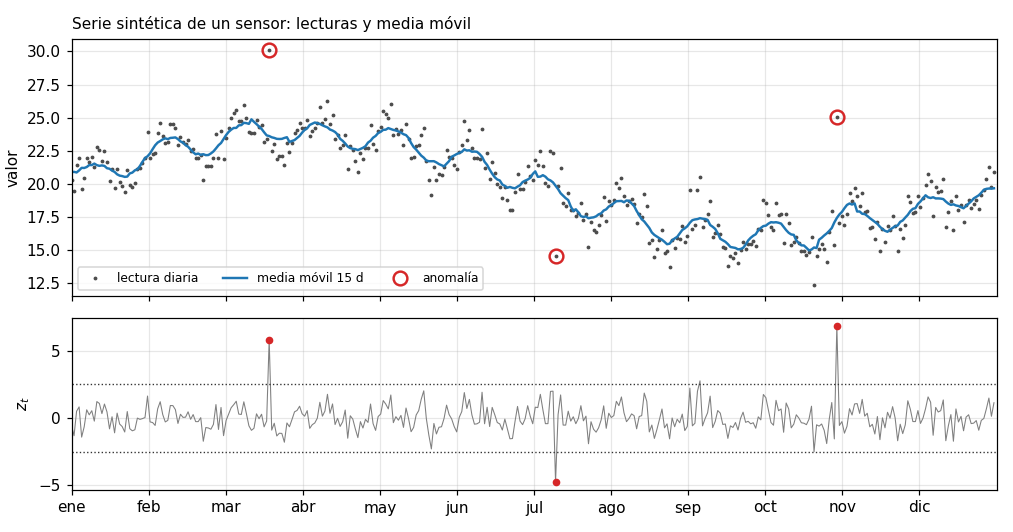
\includegraphics[width=\linewidth]{figs/demo-figura}
  \end{minipage}
\end{frame}

% ------------------------------------------------------------- 5. lista --
\begin{frame}{Lista}
  \panelheading{Supuestos del detector}

  \begin{itemize}
    \item Anomalías puntuales y de corta duración.
    \item Sin tendencia dentro de la ventana.
    \item Lecturas independientes entre sensores.
    \item Ausencia de huecos largos en la serie.
  \end{itemize}

  El primero es el que justifica la ventana [t-30, t-1]: se asume que la
  anomalía es un pico aislado y no el inicio de un periodo prolongado de
  deriva.
\end{frame}

% ------------------------------------------------------------- 6. tabla --
\subsection{Tablas}

\begin{frame}{Tabla}
  \panelheading{Estimaciones}

  \begin{tabular}{@{}lrrr@{}}
    \toprule
    Umbral        & Precisión & Exhaustividad & $F_1$ \\
    \midrule
    $z > 2{,}0$   & 0,71  & 0,88  & 0,79 \\
    $z > 2{,}5$   & 0,82  & 0,79  & 0,80 \\
    $z > 3{,}0$   & 0,91  & 0,61  & 0,73 \\
    $z > 3{,}5$   & 0,95  & 0,42  & 0,58 \\
    \bottomrule
  \end{tabular}

  Estimadas por validación cruzada sobre las 312 particiones con anomalías
  etiquetadas.
\end{frame}

% ==========================================================================
%  DIAPOSITIVA A DOS FILAS
% ==========================================================================
\section{Dos filas}

% ------------------------------------------------------ 1. un párrafo por fila --
\subsection{Texto}

\begin{frame}{Un párrafo por fila}
\begin{tworows}
  El detector por ventana deslizante compara cada lectura con las de su
  entorno inmediato: la referencia se calcula sobre la propia serie, de modo
  que todo lo que varía lentamente queda absorbido por la media móvil.
\nextrow
  Esto elimina la necesidad de un modelo explícito de la señal y neutraliza
  las derivas lentas del sensor, a costa de perder las anomalías que se
  extienden más allá del tamaño de la ventana.
\end{tworows}
\end{frame}

% ------------------------------------------- 2. cabecera y varios párrafos --
\begin{frame}{Con cabecera y varios párrafos}
\begin{tworows}
  \panelheading{Contexto}

  Los métodos clásicos de detección de anomalías en series temporales
  ajustan un modelo de la señal y señalan como anómalas las lecturas que se
  alejan de la predicción, con un coste de ajuste que hay que repetir para
  cada sensor.

  Concluyen que la mayor parte de las anomalías reales son puntuales y de
  corta duración.
\nextrow
  \panelheading{Este trabajo}

  Aquí se comprueba si empleando \textbf{únicamente} una media móvil y un
  umbral sobre el residuo se recupera esa misma capacidad de detección.

  El detector es un \emph{z-score} sobre ventana deslizante con las mismas
  ventanas temporales y el umbral fijado por validación cruzada sobre
  particiones del histórico.
\end{tworows}
\end{frame}

% -------------------------------- 3. texto y figura a la derecha en cada fila --
\subsection{Figuras}

\begin{frame}{Texto y figura en cada fila}
\begin{tworows}
  \begin{minipage}[t]{0.48\linewidth}\vspace{0pt}\ucmbodysetup
    \panelheading{Señal diaria}
    Lectura diaria de un sensor sintético con su media móvil de 15 días,
    agregada sobre los 12 sensores de la instalación.
  \end{minipage}\hfill
  \begin{minipage}[t]{0.48\linewidth}\vspace{0pt}
    \ucmfigure{figs/demo-figura}
  \end{minipage}
\nextrow
  \begin{minipage}[t]{0.48\linewidth}\vspace{0pt}\ucmbodysetup
    \panelheading{Anomalías detectadas}
    Residuo normalizado por fecha, sobre el mismo periodo y los mismos
    sensores; los puntos marcados superan el umbral.
  \end{minipage}\hfill
  \begin{minipage}[t]{0.48\linewidth}\vspace{0pt}
    \ucmfigure{figs/demo-figura}
  \end{minipage}
\end{tworows}
\end{frame}

% ------------------------------------------ 4. texto arriba, figura abajo --
\begin{frame}{Texto arriba, figura abajo}
\begin{tworows}
  \panelheading{Particiones}

  Las particiones se definen por sensor $\times$ año $\times$ trimestre. De
  las 480 resultantes, 312 contienen al menos una anomalía etiquetada; el
  resto no aporta información a la validación y se descarta.

  La distribución de anomalías por partición es muy asimétrica: la mediana
  es de 2 y la cola llega hasta varias decenas.
\nextrow
  \ucmfigure{figs/demo-figura}
\end{tworows}
\end{frame}

% -------------------------------------------------------- 5. lista y texto --
\begin{frame}{Lista en una fila}
\begin{tworows}
  \panelheading{Supuestos}

  \begin{itemize}
    \item Anomalías puntuales y de corta duración.
    \item Sin tendencia dentro de la ventana.
    \item Lecturas independientes entre sensores.
  \end{itemize}
\nextrow
  \panelheading{Consecuencias}

  El primer supuesto es el que justifica la ventana [t-30, t-1]: se asume
  que la anomalía es un pico aislado y no el inicio de un periodo prolongado
  de deriva. El segundo obliga a particionar por trimestre además de por
  año, porque la señal tiene un ciclo anual marcado.
\end{tworows}
\end{frame}

% -------------------------------------------------------------- 6. tabla --
\subsection{Tablas}

\begin{frame}{Tabla en una fila}
\begin{tworows}
  \panelheading{Estimaciones}

  \begin{tabular}{@{}lrrr@{}}
    \toprule
    Umbral        & Precisión & Exhaustividad & $F_1$ \\
    \midrule
    $z > 2{,}0$   & 0,71  & 0,88  & 0,79 \\
    $z > 2{,}5$   & 0,82  & 0,79  & 0,80 \\
    $z > 3{,}0$   & 0,91  & 0,61  & 0,73 \\
    $z > 3{,}5$   & 0,95  & 0,42  & 0,58 \\
    \bottomrule
  \end{tabular}
\nextrow
  \panelheading{Lectura}

  Solo los dos umbrales intermedios equilibran precisión y exhaustividad.
  El umbral más alto apenas produce falsos positivos, pero deja pasar más de
  la mitad de las anomalías.
\end{tworows}
\end{frame}

% --------------------------------------------------------- 7. tabla ancha --
\begin{frame}{Tabla ancha en una fila}
\begin{tworows}
  \panelheading{Sensibilidad de la ventana}

  \begin{tabular}{@{}lrrrrrrr@{}}
    \toprule
    Ventana & Particiones & Lecturas & Precisión & IC inf. & IC sup. & Exhaust. & $F_1$ \\
    \midrule
    (t-7, t-1)   & 312 & 52\,560 & 0,74 & 0,67 & 0,81 & 0,83 & 0,78 \\
    (t-30, t-1)  & 312 & 52\,560 & 0,82 & 0,76 & 0,88 & 0,79 & 0,80 \\
    (t-60, t-1)  & 312 & 52\,560 & 0,80 & 0,73 & 0,86 & 0,75 & 0,77 \\
    (t-90, t-1)  & 312 & 52\,560 & 0,72 & 0,65 & 0,79 & 0,70 & 0,71 \\
    \bottomrule
  \end{tabular}
\nextrow
  \panelheading{Tabla más ancha que la fila}

  \begin{tabular}{@{}lrrrrrrrrrr@{}}
    \toprule
    Umbral & Sensores & Días & Lecturas & Precisión & IC inf. & IC sup. & Exhaust. & $F_1$ & FP & $n$ \\
    \midrule
    $z > 2{,}5$ & 12 & 4380 & 52\,560 & 0,82 & 0,76 & 0,88 & 0,79 & 0,80 & 41 & 312 \\
    $z > 3{,}0$ & 12 & 4380 & 52\,560 & 0,91 & 0,86 & 0,95 & 0,61 & 0,73 & 14 & 312 \\
    $z > 3{,}5$ & 12 & 4380 & 52\,560 & 0,95 & 0,90 & 0,98 & 0,42 & 0,58 &  5 & 312 \\
    \bottomrule
  \end{tabular}
\end{tworows}
\end{frame}

% ------------------------------------------- 8. tabla que desborda la fila --
\begin{frame}{Tabla que no cabe}
\begin{tworows}
  \panelheading{Tal cual: se sale de la diapositiva}

  \begin{tabular}{@{}lrrrrrrrrrrrr@{}}
    \toprule
    Umbral & Sensores & Días & Lecturas & Particiones & Precisión & IC inf. & IC sup. & Exhaust. & $F_1$ & FP & FN & AUC \\
    \midrule
    $z > 2{,}5$ & 12 & 4380 & 52\,560 & 312 & 0,82 & 0,76 & 0,88 & 0,79 & 0,80 & 41 & 49 & 0,912 \\
    $z > 3{,}0$ & 12 & 4380 & 52\,560 & 312 & 0,91 & 0,86 & 0,95 & 0,61 & 0,73 & 14 & 91 & 0,904 \\
    $z > 3{,}5$ & 12 & 4380 & 52\,560 & 312 & 0,95 & 0,90 & 0,98 & 0,42 & 0,58 &  5 & 135 & 0,887 \\
    \bottomrule
  \end{tabular}
\nextrow
  \panelheading{La misma con \texttt{\textbackslash resizebox}}

  \resizebox{\linewidth}{!}{%
  \begin{tabular}{@{}lrrrrrrrrrrrr@{}}
    \toprule
    Umbral & Sensores & Días & Lecturas & Particiones & Precisión & IC inf. & IC sup. & Exhaust. & $F_1$ & FP & FN & AUC \\
    \midrule
    $z > 2{,}5$ & 12 & 4380 & 52\,560 & 312 & 0,82 & 0,76 & 0,88 & 0,79 & 0,80 & 41 & 49 & 0,912 \\
    $z > 3{,}0$ & 12 & 4380 & 52\,560 & 312 & 0,91 & 0,86 & 0,95 & 0,61 & 0,73 & 14 & 91 & 0,904 \\
    $z > 3{,}5$ & 12 & 4380 & 52\,560 & 312 & 0,95 & 0,90 & 0,98 & 0,42 & 0,58 &  5 & 135 & 0,887 \\
    \bottomrule
  \end{tabular}}
\end{tworows}
\end{frame}

% ==========================================================================
%  SIMBOLOS MATEMATICOS Y CARACTERES ESPECIALES
% ==========================================================================
\section{Símbolos}

\subsection{Matemáticas}

\begin{frame}{Matemáticas en línea y desplegadas}
\begin{twocols}
  \panelheading{En línea}

  El residuo $r_t = y_t - \hat\mu_t$ tiene desviación típica $\hat\sigma_t$,
  de modo que $z_t = r_t / \hat\sigma_t$ y su intervalo de normalidad es
  $\hat\mu_t \pm 2{,}5\,\hat\sigma_t$.

  Con $\alpha = 0{,}05$, se marca una anomalía si $|z_t| > z_{1-\alpha/2}$;
  aquí $z_{1-\alpha/2} = 1{,}96 < 2{,}5$.

  Griegas: $\alpha\,\beta\,\gamma\,\delta\,\varepsilon\,\theta\,\lambda\,\mu\,
  \pi\,\rho\,\sigma\,\tau\,\phi\,\chi\,\psi\,\omega$ y
  $\Gamma\,\Delta\,\Theta\,\Lambda\,\Xi\,\Pi\,\Sigma\,\Phi\,\Psi\,\Omega$.

  Relaciones: $a \le b$, $c \ge d$, $x \ne y$, $u \approx v$,
  $n \to \infty$, $A \subset B$, $z \in \mathbb{R}$, $\forall i\ \exists j$.
\nextcol
  \panelheading{Desplegadas}

  \[
    \hat\mu_t = \frac{1}{w} \sum_{k=1}^{w} y_{t-k}
  \]

  \[
    \hat\sigma_t^2 = \frac{1}{w-1} \sum_{k=1}^{w}
      \left( y_{t-k} - \hat\mu_t \right)^2
  \]

  \[
    F_1 = \frac{2\,PR}{P + R},
    \qquad
    \bar x = \frac{1}{n}\sum_{i=1}^{n} x_i
  \]
\end{twocols}
\end{frame}

\begin{frame}{Ecuaciones con estructura}
\begin{twocols}
  \panelheading{Sistema alineado}

  \begin{align*}
    y_t           &= \mu_t + \varepsilon_t \\
    \varepsilon_t &\sim \mathcal{N}(0, \sigma^2) \\
    a_t           &= \mathbb{1}\{|z_t| > \tau\}
  \end{align*}

  \panelheading{Por casos}

  \[
    a_t =
    \begin{cases}
      1 & \text{si } |z_t| > \tau \text{ en } [t-30,\, t-1],\\
      0 & \text{en otro caso.}
    \end{cases}
  \]
\nextcol
  \panelheading{Matriz e integral}

  \[
    \Sigma =
    \begin{pmatrix}
      \sigma_1^2 & \rho\sigma_1\sigma_2 \\
      \rho\sigma_1\sigma_2 & \sigma_2^2
    \end{pmatrix}
  \]

  \[
    \Phi(z) = \int_{-\infty}^{z}
      \frac{1}{\sqrt{2\pi}}\, e^{-t^2/2}\, \mathrm{d}t
  \]

  \[
    \frac{\partial \ell}{\partial \tau} = 0,
    \qquad
    \nabla^2 \ell \prec 0
  \]
\end{twocols}
\end{frame}

\subsection{Caracteres}

\begin{frame}{Caracteres especiales y tipografía}
\begin{twocols}
  \panelheading{Español}

  Acentos y diéresis: á é í ó ú Á É Í Ó Ú ü Ü ñ Ñ.
  Signos de apertura: ¿Cuántos? ¡Ojo!
  Ordinales: 1.º, 2.ª, n.º 5.

  Comillas: «angulares», “inglesas”, ‘simples’.
  Rayas: guion-, semirraya –, raya —.
  Puntos suspensivos… y ligaduras: fi fl ffi.

  \panelheading{Símbolos sueltos}

  En texto: © ® ™ § ¶ † ‡ • · … ‰ ° ª º № € \$ £ ¥ µ Ω Å

  En modo matemático:
  $\pm\ \times\ \div\ \neq\ \leq\ \geq\ \approx\ \infty\ \sqrt{x}\ \sum\ \prod\
  \int\ \partial\ \nabla\ \in\ \subset\ \forall\ \exists\ \to\ \Rightarrow\
  \leftrightarrow$
\nextcol
  \panelheading{Unidades y notación}

  Longitud: 12,5\,mm; masa: 3,2\,kg; frecuencia de muestreo: 50\,Hz;
  tensión: 3,3\,V.

  Tasas: 1,8 anomalías por 10\textsuperscript{3} lecturas;
  95\,\% IC; p\,<\,0,001; 2,5\,‰.

  \panelheading{Monoespaciado}

  \texttt{sensor == "s07" \& mes \textbackslash in 6:9}

  \texttt{z = (y - mu) / sigma \# umbral 2.5}
\end{twocols}
\end{frame}

\subsection{Enlaces}

% ------------------------------------------------------ enlaces y notas --
\begin{frame}{Enlaces y notas al pie}
\begin{twocols}
  \panelheading{Direcciones web}

  Enlace explícito: \url{https://www.uc3m.es/inicio}.

  Enlace con texto: la plantilla la mantiene la
  \href{https://www.uc3m.es}{Universidad Carlos III de Madrid} y el tema
  visual sigue la identidad del
  \href{https://www.isciii.es}{Instituto de Salud Carlos III}.

  Correo: \href{mailto:nadie@uc3m.es}{nadie@uc3m.es}.

  \panelheading{Referencias internas}

  Las entradas del índice de sección son enlaces internos y conservan el
  color de la plantilla: solo se tiñen las URL y las citas.
\nextcol
  \panelheading{Notas al pie}

  La detección de anomalías por ventana deslizante es uno de los métodos
  más antiguos y sencillos\footnote{Chandola, Banerjee y Kumar,
  \emph{ACM Comput. Surv.} 41(3), 2009.} y elimina así la necesidad de
  ajustar un modelo de la señal.

  \panelheading{Numeración}

  El pie de las diapositivas de contenido lleva el número de diapositiva y el
  total. La portada y los índices de sección van con \texttt{[plain]} y
  \texttt{[noframenumbering]}, así que ni llevan pie ni cuentan.
\end{twocols}
\end{frame}

\end{document}
